\documentclass[a4paper]{article}
\usepackage{amsmath}
\usepackage{amssymb}
\usepackage{xcolor}
\usepackage{amsthm}
\usepackage{dsfont}
\usepackage{graphicx}
\usepackage{hyperref}

\usepackage[margin=3.8cm, top=3cm, bottom=3cm]{geometry}

\author{Jeroen van Riel}
\date{\monthyeardate\today}
\title{Optimal Control Notes}

\begin{document}

\section*{Videos}

\begin{itemize}
  \item \textbf{4 (9/2/2020)} -- Explanation of ``necessary conditions does not \textit{follow} from (1.27)'' (around 1:00:00).
  \item \textbf{5 (9/8/2020)} -- Question about uniqueness of first and second variation.
  \item \textbf{6 (9/10/2020)} -- Preview discussion of Section 2.3.
  \item \textbf{7 (9/15/2020)} --
\end{itemize}



\section{Introduction}

\subsection*{1.2.1 -- Unconstrained optimization}

First-order necessary condition for optimality (stationary point, Fermat's theorem):
\begin{align*}
  \nabla f(x^{*}) = 0 .
\end{align*}
%
Second-order necessary condition for optimality (positive semidefinite Hessian):
\begin{align*}
  \nabla^{2} f(x^{*}) \geq 0 .
\end{align*}
%
Second-order sufficient condition for optimality:
If $f \in \mathcal{C}^{2}$ satisfies
\begin{align*}
  \nabla f(x^{*}) = 0 \quad \text{ and } \quad \nabla^{2} f(x^{*}) > 0 ,
\end{align*}
on an interior point $x^{*} \in D$, then $x^{*}$ is a strict local minimum of
$f$.


\subsubsection*{Exercise 1.1}

We say $d$ is a feasible direction at $x^{*}$, if it is of unit length and there
exists some $\delta > 0$ such that $x^{*} + \alpha d \in D$ for all
$0 \leq \alpha \leq \delta$. As discussed after the exercise description, it is
possible that $x^{*} \in D$, but there are no feasible directions. This shows
that we need some restrictions on $D$ in order for the statement to hold. We say
that $D$ is \textit{locally star-shaped} if there exists some $\delta^{*} > 0$
such that every $x \in D \cap B(x^{*}, \delta^{*})$ satisfies
$x = x^{*} + \alpha d$ for some feasible direction $d$ and
$0 \leq \alpha < \delta^{*}$, see Figure~\ref{fig:star-shaped-domain}.
%
For every feasible direction $d$, we have
\begin{align*}
  f(x^{*} + \alpha d) &= f(x^{*}) + \alpha \nabla f(x^{*}) \cdot d + \frac{1}{2}d^{T}\nabla^{2}f(x^{*})d \alpha^{2} + o(a^{2}) \\
  &\geq f(x^{*}) + \frac{1}{2}d^{T}\nabla^{2}f(x^{*})d \alpha^{2} + o(a^{2}) \\
  &> f(x^{*}) ,
\end{align*}
where the last inequality follows again by taking $\alpha$ sufficiently small.
%
Recall that $o(\alpha^{2})$ and the corresponding value of $\epsilon$ in the
proof for the unconstrained case depend on the choice of $d$. When the set of
all feasible $d$ is compact, the Weierstrass Theorem again tells us that we can
take the minimum of $\epsilon$ over all $d$.
%
In that case, $x^{*}$ is a local minimum.

When the set of all feasible directions is not not compact, I am not completely
sure how to proceed. Assuming convexity of $D$ will not help, because
$D \cap B(x^{*}, \delta^{*})$ can then still be an open star-shaped domain.
I think that we should somehow use the continuity of $f$.

\begin{figure}[b]
  \centering
  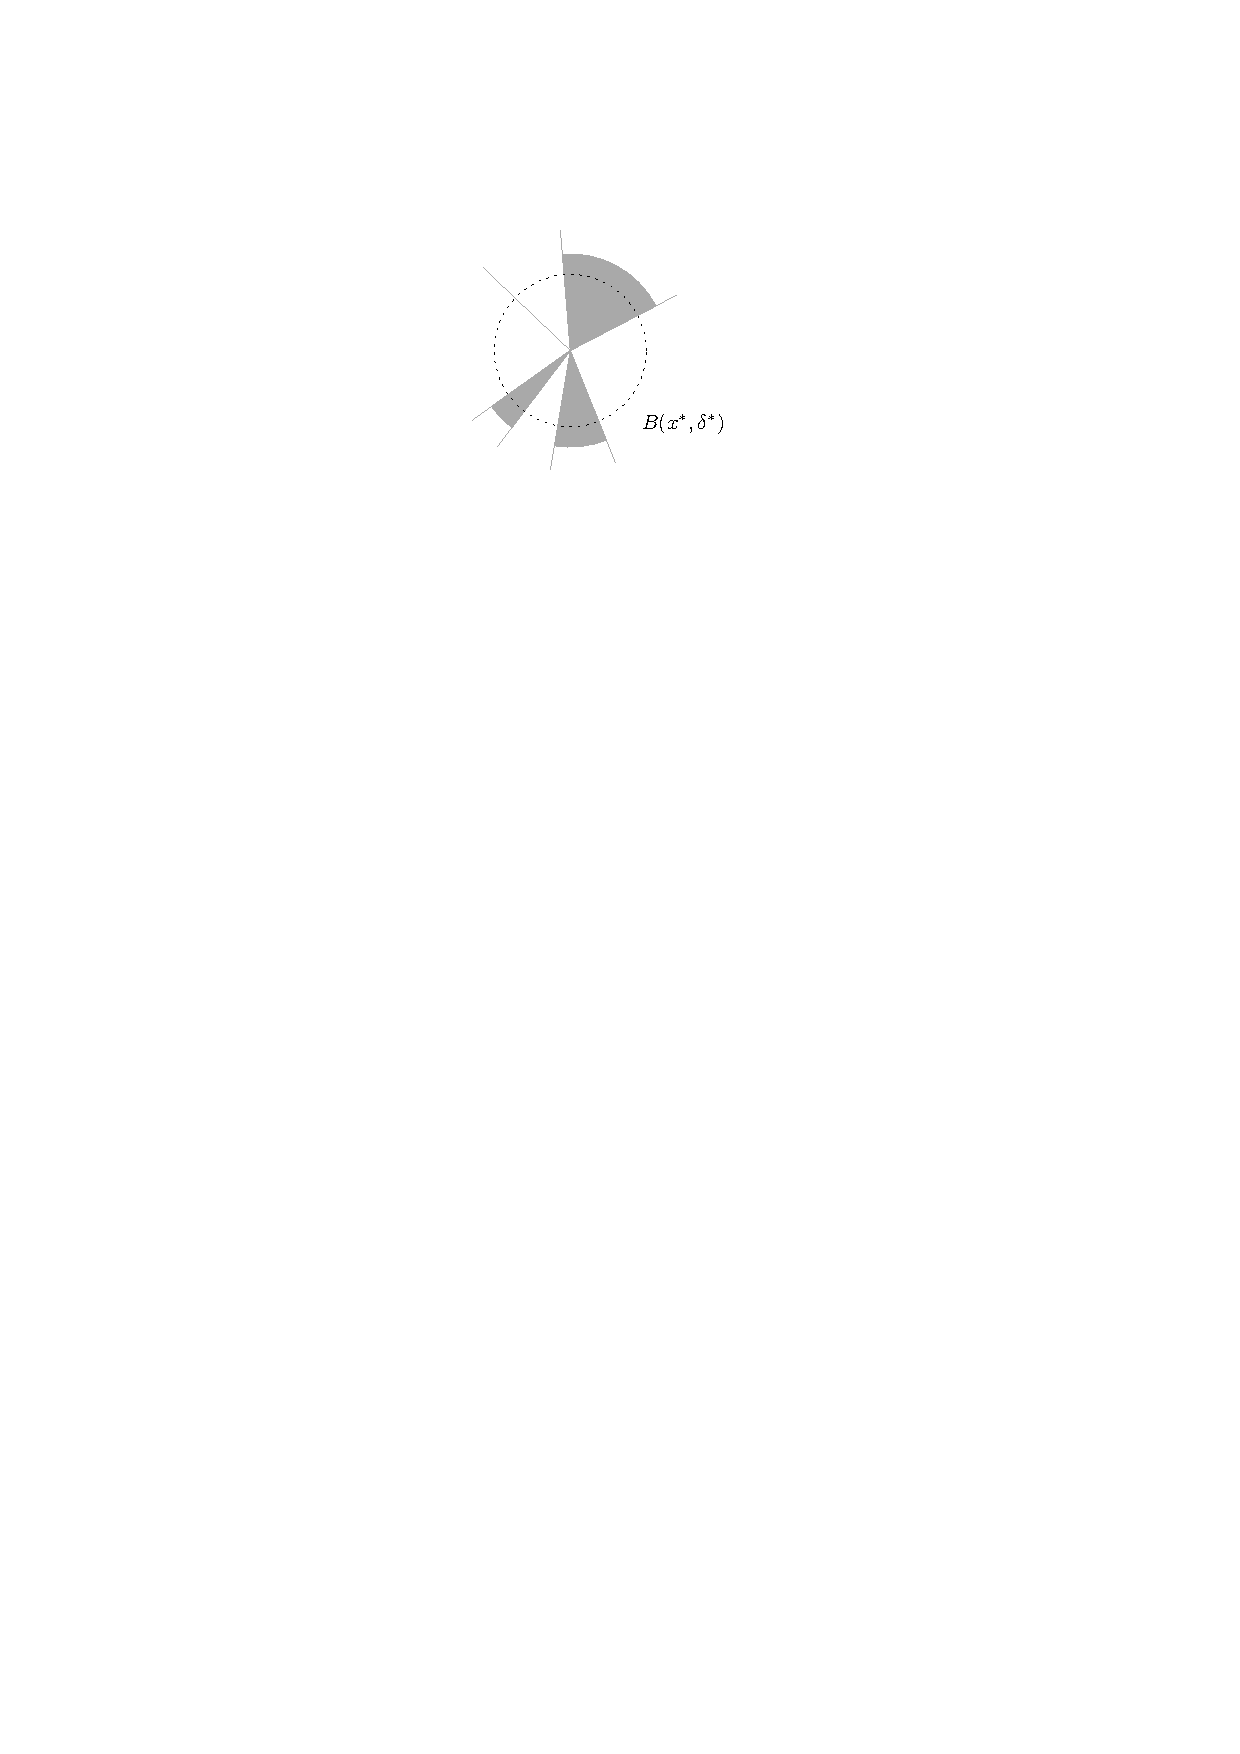
\includegraphics[]{figures/notes/locally-star-shaped}
  \caption{Domain $D$ indicated in grey. Note that subsets of feasible
    directions can be either open or closed. A single isolated feasible
    direction is also drawn.}
  \label{fig:star-shaped-domain}
\end{figure}


\subsection*{1.2.2 -- Constrained optimization}

\subsubsection*{Exercise 1.2}

Consider the following example in dimension $n=3$. Define
\begin{align*}
  h_{1}(x, y, z) &= z , \\
  h_{2}(x, y, z) &= z - y^{2} ,
\end{align*}
such that $D$ is the $x$-axis and we have
\begin{align*}
  \nabla h_{1}(0) = \nabla h_{2}(0) = (0, 0, 1) ,
\end{align*}
which shows that $x^{*} = 0$ is not a regular point. Now define
$f(x,y,z) = x^{2} + y$ such that $\nabla f(0) = (0, 1, 0) \perp (0, 0, 1)$,
which shows that (1.24) cannot hold.


\subsubsection*{Augmented cost function}

The \textit{augmented cost} function is defined as
\begin{align*}
  \ell(x,\lambda) := f(x) + \sum_{i=1}^{m} \lambda_{i}h_{i}(x) ,
\end{align*}
with gradient given by
\begin{align*}
  \nabla \ell(x, \lambda) = \begin{pmatrix} \ell_{x}(x, \lambda) \\ \ell_{\lambda}(x, \lambda) \end{pmatrix} = \begin{pmatrix} \nabla f(x) + \sum_{i=1}^{m} \lambda_{i} \nabla h_{i}(x) \\[0.3em] h(x) \end{pmatrix} .
\end{align*}
%
If $x^{*}$ is a local constrained minimum of $f$ and $\lambda^{*}$ is the
corresponding vector of Lagrange multipliers for which the first order necessary
condition (1.24) holds, then $\nabla \ell(x^{*}, \lambda^{*}) = 0$.

On page 16, it is stated that ``However, it does \textit{not} follow that (1.27)
is a necessary condition for $x^{*}$ to be a constrained minimum of $f$.'' This
is confusing me, because (1.27) does hold under the stated assumptions.
Maybe the author wants to stress the fact that the regularity assumption is required.


\subsection*{1.3.2 -- First variation and first-order necessary condition}

\subsubsection*{Exercise 1.5}

Let $\eta \in V$ be arbitrary and define $g_{\eta}$ like in the text, so
$g_{\eta}(\alpha) = J(y + \alpha \eta)$. We can differentiate it as a function of
$\alpha$, which yields
\begin{align*}
  g_{\eta}'(\alpha) &= \frac{d}{d\alpha}  \int_{0}^{1} \phi(y(x) + \alpha \eta(x)) dx \\
  &= \int_{0}^{1} \frac{d}{d\alpha} \phi(y(x) + \alpha \eta(x)) dx  \\
  &= \int_{0}^{1} \phi'(y(x) + \alpha \eta(x)) \eta(x) dx .
\end{align*}
In the first step, we used Leibniz integral rule for differentiation under the integral sign, which is allowed because $(x,\alpha) \mapsto \phi(y(x) + \alpha \eta(x))$ is continuous in both variables.
We obtain the desired result by evaluating $\delta J |_{y}(\eta) = g_{\eta}'(0)$.

\subsubsection*{Exercise 1.6}

First, observe that we can obtain an equivalent definition of the second
variation, like the Gateaux derivative (1.33) was equivalent to the first
variation, by using the definition of $o(\alpha^{2})$ to rewrite the expansion
(1.38) to
\begin{align*}
  \delta^{2}J |_{y}(\eta) = \lim_{\alpha \rightarrow 0} \frac{J(y + \alpha \eta) - J(y) - \delta J |_{y}(\eta) \alpha}{\alpha^{2}} .
\end{align*}
By comparing this to the Taylor expansion of $g_{\eta}$ around $0$, given by
\begin{align*}
  g_{\eta}(\alpha) = g_{\eta}(0) + \alpha g'_{\eta}(0) + \frac{\alpha^{2}}{2} g''_{\eta}(0) + o(\alpha^{2}) ,
\end{align*}
which is equivalently stated as
\begin{align*}
  \lim_{\alpha \rightarrow 0} \frac{g_{\eta}(\alpha) - g_{\eta}(0) - \alpha g'_{\eta}(0)}{\alpha^{2}} = \frac{1}{2} g''_{\eta}(0) ,
\end{align*}
we conclude that
\begin{align*}
  \delta^{2} J |_{y}(\eta) = g''_{\eta}(0) / 2 .
\end{align*}
Note this factor two difference because expansion (1.38) is not exactly analogous to the regular Taylor expansion.
%
Because $\phi$ is twice differentiable, the map
$(x, \alpha) \mapsto \phi'(y(x) + \alpha \eta(x)) \eta(x)$ is continuous in both
arguments, so we can again use Leibniz integral rule to compute
\begin{align*}
  g_{\eta}''(\alpha) = \frac{d}{d\alpha} g_{\eta}'(\alpha) &= \frac{d}{d\alpha} \int_{0}^{1} \phi'(y(x) + \alpha\eta(x))\eta(x) dx \\
  &= \int_{0}^{1} \frac{d}{d\alpha} \phi'(y(x) + \alpha \eta(x))\eta(x) dx \\
  &= \int_{0}^{1} \phi''(y(x) + \alpha \eta(x))\eta^{2}(x) dx ,
\end{align*}
which we evaluate at zero to conclude
\begin{align*}
  \delta^{2}J |_{y}(\eta) = g_{\eta}''(0) / 2 = \frac{1}{2} \int_{0}^{1} \phi''(y(x))\eta^{2}(x) dx .
\end{align*}
%
It is easily seen that this is indeed a quadratic form, by writing $\delta^{2}J |_{y}(\eta) = B(\eta, \eta) / 2$, with functional $B: V \times V \rightarrow \mathbb{R}$ defined as
\begin{align*}
  B(\eta_{1}, \eta_{2}) = \int_{0}^{1} \phi''(y(x)) \eta_{1}(x) \eta_{2}(x) dx ,
\end{align*}
which is bilinear because $B(\eta_{1}, \eta_{2}) = B(\eta_{2}, \eta_{1})$ and
\begin{align*}
  B(\alpha \eta_{1} + \beta \eta_{2}, \xi) &= \int_{0}^{1} \phi''(y(x)) (\alpha \eta_{1}(x) + \beta \eta_{2}(x)) \xi(x) dx \alpha \\
  &= \alpha \int_{0}^{1} \phi''(y(x)) \eta_{1}(x) \xi(x) dx + \beta \int_{0}^{1} \phi''(y(x)) \eta_{2}(x) \xi(x) dx \\
  &= \alpha B(\eta_{1}, \xi) + \beta B(\eta_{2}, \xi) .
\end{align*}


\section{Calculus of Variations}

\subsubsection*{Exercise 2.3}

%
We define the \textit{remainder} of $L$ at some point $p \in [0,1] \times \mathbb{R}^{2}$ with some
perturbation $h$ as
\begin{align*}
  R(p, h) = L(p + h) - L(p) - dL(p) \cdot h ,
\end{align*}
where $dL(p)$ is the differential of $L$ at $p$.
%
Whenever $dL(p)$ exists at $p$, Taylor's theorem for multivariable functions tells us that
\begin{align}
  \label{eq:taylor_remainder_convergence}
  \frac{R(p, h)}{\| h \|} \longrightarrow 0 \quad \text{ as } h \rightarrow 0,
\end{align}
where we write $\| h \|$ for the usual Euclidean norm.
%
Consider a sequence of functions $(\eta_{n})$ such that $\lim_{n \to \infty} \| \eta_{n} \|_{1} = 0$ with respect to the 1-norm defined in (1.30).
%
Now define
$h_{n}(x) =(0, \eta_{n}(x), \eta_{n}'(x))$, then by H\"{o}lder's inequality, we
have
\begin{align*}
  \| h_{n}(x) \| &\leq \| h_{n} (x) \|_{1} \\
                                                               & \leq \sup_{x \in [0,1]} |\eta_{n}(x)| + \sup_{x \in [0,1]} | \eta_{n}'(x) | \\
  &= \| \eta_{n} \|_{1} ,
\end{align*}
which means that we have $\lim_{n \to \infty} \|h_{n}(x)\| = 0$ for every $x \in [0, 1]$.
%
Now define $p(x)=(x,y(x),y'(x))$, % $R_{n}(x) = R((x, y(x), y'(x)), h_{n}(x))$,
then we have
\begin{subequations}
  \label{eq:bound}
\begin{align}
  \frac{1}{\| \eta_{n} \|_{1}}\int_{a}^{b} R(p(x), h_{n}(x)) dx &\leq (b-a) \sup_{x \in [0, 1]} \; \frac{R(p(x), h_{n}(x))}{\| \eta_{n} \|_{1}} \\
  & \leq (b-a) \sup_{x \in [0,1]} \; \underbrace{\frac{R(p(x), h_{n}(x))}{\|h_{n}(x)\|}}_{P_{n}(x) :=} .
\end{align}
\end{subequations}
Let $\epsilon > 0$ be given, then for every $x \in [0, 1]$ there is some $N(x)$ such that $P_{n}(x) < \epsilon$ for all $n \geq N(x)$.
Since the interval $[0, 1]$ is compact, the Weierstrass theorem gives us $N = \max_{x \in [0,1]} N(x)$ such that
\begin{align*}
  \sup_{x \in [0, 1]} P_{n}(x) < \epsilon \quad \text{ for all } n \geq N .
\end{align*}
This shows that the left-hand side of~\eqref{eq:bound} goes to zero as $n \rightarrow \infty$.
%
To conclude, observe that $\delta J|_{y}(\eta_{n})$ defined by (2.14) satisfies
the definition of (1.37), because we have shown that
\begin{align*}
  J(y + \eta_{n}) - J(y) - \delta J|_{y}(\eta_{n}) = \int_{a}^{b} R(p(x), h_{n}(x)) dx = o(\| \eta_{n} \|_{1}) .
\end{align*}
%
{\color{blue} Also true for 0-norm?}

For the 0-norm, the above proof does not go through, because it is not too difficult
to construct a sequence $(\eta_{n})$ like $y_{2}$ in Figure 2.6 such that
$\lim_{n \to \infty} \|\eta_{n}\|_{0} = 0$, but which has
$\sup_{x \in [0,1]} \eta_{n}'(x) \geq C$ for all $n$, with some constant
$C > 0$.
This means that $\|h_{n}(x)\|$ will not converge to zero as $n \to \infty$.


\end{document}
